% https://github.com/abdur75648/Deep-Learning-Specialization-Coursera/blob/main/Neural%20Networks%20and%20Deep%20Learning/Week2/Logistic%20Regression%20as%20a%20Neural%20Network/Logistic_Regression_with_a_Neural_Network_mindset_v6a.ipynb

\documentclass{article}
\usepackage{amssymb}
\usepackage{amsmath}
\usepackage{booktabs}
\usepackage{mathpartir}
\usepackage{tikz}
\usetikzlibrary{external}
\tikzexternalize
\usepackage{pgfplots}
\newcommand\code[1]{\texttt{#1}}
\begin{document}

\section{Notations}
\begin{itemize}
  \item $X$ = feature matrix
  \item $n_x$ = dimension (ie, size) of feature vector
  \item $M_{train}$ = Size of train dataset
  \item $M_{test}$ = Size of test dataset
  \item $M$ = Size of entire dataset ($M_{train} + M_{test}$)
  \item Label assigned to a data element = $y$
  \begin{itemize}
    \item $y \in {0,1}$ for binary classification
  \end{itemize}
  \item Label assigned to entire dataset = $Y \in \mathbb{R}^{1 \times M}$
  \begin{itemize}
    \item \code{Y.shape = (1, M)}
  \end{itemize}
  \item $\hat{y}$: predicted label
  \item $x^{(i)}$: i-th element in a vector
  \item $L$: loss function
  \item $J$: cost function
  \item $\alpha$: learning rate
\end{itemize}

\section{Logistic regression}
\begin{itemize}
  \item For binary classification
  \item Can be viewed as a tiny neural network ??
  \item Unlike linear regression, the line seperating classes can
    'bend'
  \begin{itemize}
    \item Hence the term 'logistic' instead of 'linear'
  \end{itemize}
  \item Each data element is an n-dimensional \emph{feature vector}
  \item All feature vectors may be stacked together (as columns
    preferably) to get a \emph{feature matrix} ($X$)
  \item $x \in \mathbb{R}^{n_x}$ for each $x \in X$
  \item Split available dataset into \emph{training and test data}
  \item Training: Instead of looping, consider all data points at once.
  \item $\hat{y} = P(y=1 | x)$: Probaby that label is $1$ given that
    input is $x$
  \begin{itemize}
    \item $\hat{y}$ being a probability means $\hat{y} \in [0, 1]$
  \end{itemize}
  \item Parameters of logistic regression:
  \begin{itemize}
    \item Weights: $w \in \mathbb{R}^{n_x}$
    \item Bias: $b \in \mathbb{R}$
  \end{itemize}
  \item Aim of logistic regression is to learn the values for these
    parameters so that error is minimum
  \item Error = difference between $\hat{y}$ and $y$
  \item Some resources consider $b$ to be $w_0$, we consider $b$ to be separate.
  \item Activation function that we use: Sigmoid function (See Section~\ref{sec:sigmoid-fn}).
\end{itemize}

\subsection{Cost function for logistic regression}
Training data consists of input vectors and their correct labels.
If size of training data is $m$, the data would be like:

\begin{mathpar}
  \{
   (x^{(1)}, y^{(1)}),
   (x^{(2)}, y^{(2)}),
   ...,
   (x^{(m)}, y^{(m)})
  \}
\end{mathpar}


\begin{center}
\begin{tabular}{lll}
  \toprule
  Description    & Symbol & Dimensions     \\
  \midrule
  Weights        & w      & $n_x \times 1$ \\
  %Weights        & w      & $1 \times n_x$ \\
  Feature vector & x      & $n_x \times 1$ \\
  Feature matrix & X      & $n_x \times m$ \\
  \bottomrule
\end{tabular}
\end{center}

\begin{mathpar}
  z = w^Tx + b \\
  \hat{y} = \sigma(z)
\end{mathpar}

where $\sigma$ is the sigmoid function.\\

We want our prediction $\hat{y}^{(i)}$ to be as close to $y^{(i)}$ as
possible.
ie, $\hat{y}^{(i)} \approx y^{(i)}$ is desired.
We define a loss function $L$ (See Section~\ref{sec:loss-fn}) to help
attain this.

\begin{mathpar}
  L(\hat{y}, y) = -[y.log\hat{y} + (1-y).log(1-\hat{y})]
\end{mathpar}

\begin{itemize}
 \item This function was chosen because it is convex.
 \item The graph in 3D is like a bowl
 \item That means there is no problem of getting stuck at local minima ??
\end{itemize}

\begin{itemize}
  \item Minimising the value of the loss function is an optimization problem.
  \item Loss function is for specific data elements 
  \item \emph{Cost function} is for all data elements being considered
  \begin{itemize}
    \item We use the average of all loss function values as the cost function
    \item Tells us the cost of choosing a particular set of values as parameters
  \end{itemize}
\end{itemize}

\begin{align*}
J(w, b) &= \frac{1}{m} \sum_{i=1}^{i=m} L(\hat{y}^{(i)}, y^{(i)}) \\
        &= -\frac{1}{m} \sum_{i=1}^{i=m} \left\{ y.log\hat{y} + (1-y).log(1-\hat{y}) \right\}
\end{align*}


\section{Gradient descent}
\begin{itemize}
  \item A way to figure out parameter values for which cost function
    is minimal
  \item Think of it like a ball trying to roll down to the bottom of a
    bown by its sides.
  \item Learning rate ($\alpha$): Control how big a step are we going
    to take during training
  \item Shorthand: $dw = \frac{\partial J(w)}{\partial w}$ in $\alpha.dw$
\end{itemize}

\begin{mathpar}
  w := w - \alpha. \frac{\partial J(w, b)}{\partial w} \\
  b := b - \alpha. \frac{\partial J(w, b)}{\partial b} \\
\end{mathpar}

%%% Misc

\section{Loss function} \label{sec:loss-fn}
Used to quantify the difference between prediction and actual value in
a way that the minimization of the value of this function is an
optimization problem that is convenient to tackle.
Loss functions are also known as \emph{error functions}.

A sample loss function using squared errors:

\begin{mathpar}
  L(\hat{y}, y) = \frac{1}{2} (\hat{y} - y)^{2}
\end{mathpar}

\section{Sigmoid function} \label{sec:sigmoid-fn}
aka logistic function.

\begin{mathpar}
  f(x) = \frac{1}{1+e^{-x}}
\end{mathpar}

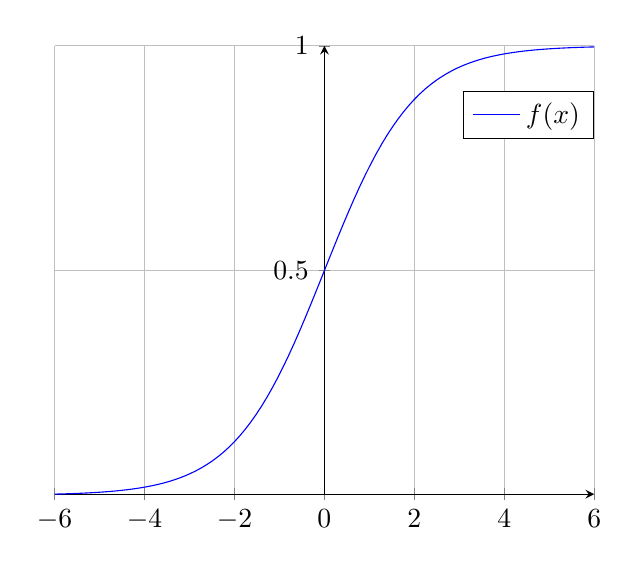
\begin{tikzpicture}[%
  declare function={%
    sigma(\x)=1/(1+exp(-\x));
    }%
]
% https://tex.stackexchange.com/questions/497949/drawing-a-sigmoid-function-and-its-derivative-in-tikz
\begin{axis}%
[
  grid=major,     
  xmin=-6,
  xmax=6,
  axis x line=bottom,
  ytick={0,.5,1},
  ymax=1,
  axis y line=middle,
  samples=100,
  domain=-6:6,
  legend style={at={(1,0.9)}}     
]
    \addplot[blue,mark=none]   (x,{sigma(x)});
    \legend{$f(x)$}
\end{axis}
\end{tikzpicture}

\begin{itemize} 
  \item Grows gently, from \emph{almost} $0$
  \item Midpoint $f(0) = 0.5$ 
  \item $y \in (0, 1)$
  \item Decays gently, \emph{towards} $1$
  \item $f(x)$ is $1$ for large positive $x$ as $e^{-x}$ tends to $0$
  \item $f(x)$ is $0$ for large negative $x$ as $e^{-x}$ gets bigger
\end{itemize} 

\section{ReLu function} \label{sec:relu-fn}

\begin{mathpar}
  f(x) = max(0, x) =
\left\{
    \begin{aligned}
         & x \quad & x > 0 \\
         & 0 \quad & x \leq 0 \\ 
    \end{aligned}
\right.
\end{mathpar}

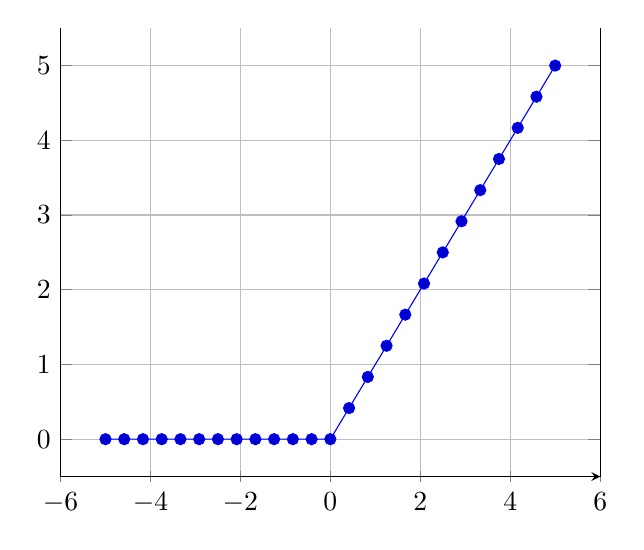
\begin{tikzpicture}
 % https://tex.stackexchange.com/questions/334588/how-to-draw-relu-function
\begin{axis}[
  grid=major,     
  xmin=-6,
  xmax=6,
  axis x line=bottom,
  %ytick={0,.5,1},
  %ymax=1,
  %domain=-3:5,
  legend style={at={(1,0.9)}}     
]
  \addplot {(x>=0)*x};
\end{axis}
\end{tikzpicture}

\begin{itemize} 
  \item Rectified Linear Unit
  \item Zero for negative values, id for others
  \item Essentially cuts off values less than zero
\end{itemize} 

\end{document}

%%% Local Variables: 
%%% TeX-command-extra-options: "-shell-escape"
%%% End: